% Gabarit pandoc des corrigés publiés (brut et guidé). Contenu sans marque ni nom de site.
% Compilation : lualatex (latexmk -lualatex).
% Le Markdown reste la source unique : ne pas éditer ce fichier .tex à la main.
\documentclass[11pt,a4paper]{article}

% --- Moteur, polices (Latin Modern) et langue ---------------------------------
\usepackage{iftex}
\ifLuaTeX\else\errmessage{Ce document se compile avec lualatex}\fi
\usepackage{amsmath,amssymb,mathtools}
\usepackage{fontspec}
% mathrm=sym : \mathrm prend ses glyphes dans la police mathématique (ℓ, μ, Ω), comme KaTeX.
\usepackage[math-style=TeX,bold-style=TeX,mathrm=sym]{unicode-math}
% Repli pour les glyphes absents de Latin Modern (indices et exposants Unicode,
% flèches, filets des schémas en texte, symboles) : DejaVu, puis Latin Modern Math
% (ℓ, lettres mathématiques Unicode des légendes).
\directlua{
  luaotfload.add_fallback("repliTexte", {"DejaVuSerif:mode=harf;", "DejaVuSans:mode=harf;", "file:latinmodern-math.otf:mode=harf;"})
  luaotfload.add_fallback("repliMono", {"DejaVuSansMono:mode=harf;", "DejaVuSans:mode=harf;", "file:latinmodern-math.otf:mode=harf;"})
}
\setmainfont{Latin Modern Roman}[RawFeature={fallback=repliTexte}]
\setsansfont{Latin Modern Sans}[RawFeature={fallback=repliTexte}]
\setmonofont{Latin Modern Mono}[RawFeature={fallback=repliMono}]
\setmathfont{Latin Modern Math}
\usepackage[french]{babel}
\frenchsetup{SmallCapsFigTabCaptions=false}

% --- Mise en page --------------------------------------------------------------
\usepackage[a4paper,margin=2.2cm,headheight=14pt,footskip=1.2cm]{geometry}
\usepackage{microtype}
\setlength{\emergencystretch}{4em}
\tolerance=1500
\setlength{\parindent}{0pt}
\setlength{\parskip}{0.55\baselineskip plus 2pt minus 1pt}
\usepackage{xcolor}
% Gris nommés : babel-french rend « ! » actif dans le document.
\definecolor{gris2}{gray}{0.98}
\definecolor{gris3}{gray}{0.97}
\definecolor{gris5}{gray}{0.95}
\definecolor{gris35}{gray}{0.65}
\definecolor{gris40}{gray}{0.60}
\definecolor{gris45}{gray}{0.55}
\definecolor{gris50}{gray}{0.50}
\definecolor{gris55}{gray}{0.45}
\definecolor{gris60}{gray}{0.40}
\definecolor{gris65}{gray}{0.35}
\definecolor{gris70}{gray}{0.30}
\definecolor{gris80}{gray}{0.20}
\definecolor{gris85}{gray}{0.15}
\usepackage{graphicx}
\usepackage{float}
\usepackage{caption}
\captionsetup{font=small,labelformat=empty,justification=centering}
\usepackage{booktabs,longtable,array,multirow,calc}
\usepackage{siunitx}
\sisetup{locale=FR}
\usepackage[version=4]{mhchem}
\usepackage{listings}
\usepackage{fancyhdr}
\usepackage{lastpage}
\usepackage[most]{tcolorbox}
\usepackage{enumitem}
\setlist{nosep,leftmargin=*,topsep=2pt}
\usepackage[hidelinks,unicode]{hyperref}
\usepackage{bookmark}
\hypersetup{pdftitle={Centrale-Supélec TSI — Sciences industrielles 2026},pdfauthor={Rédigé par IA},pdfcreator={LaTeX},pdfsubject={Corrigé brut}}
\usepackage{xurl}

% --- Pandoc : listes, tableaux, figures ----------------------------------------
\providecommand{\passthrough}[1]{#1}
\providecommand{\tightlist}{\setlength{\itemsep}{0pt}\setlength{\parskip}{0pt}}

\makeatletter
\def\maxwidth{\ifdim\Gin@nat@width>\linewidth\linewidth\else\Gin@nat@width\fi}
\def\maxheight{\ifdim\Gin@nat@height>0.55\textheight 0.55\textheight\else\Gin@nat@height\fi}
\makeatother
\setkeys{Gin}{width=\maxwidth,height=\maxheight,keepaspectratio}
\setcounter{secnumdepth}{-\maxdimen}
\providecommand{\pandocbounded}[1]{#1}
\usepackage{longtable,booktabs,array}

% --- Code (listings) -----------------------------------------------------------
\lstset{
  basicstyle=\ttfamily\small,
  columns=fullflexible,
  keepspaces=true,
  breaklines=true,
  breakatwhitespace=false,
  postbreak=\mbox{\textcolor{gris50}{$\hookrightarrow$}\space},
  frame=single,
  rulecolor=\color{gris35},
  framesep=4pt,
  xleftmargin=5pt,xrightmargin=5pt,
  backgroundcolor=\color{gris3},
  keywordstyle=\bfseries,
  commentstyle=\color{gris65},
  stringstyle=\color{gris80},
  showstringspaces=false,
  tabsize=4,
  extendedchars=true,
  aboveskip=6pt,belowskip=6pt,
}

% --- Macros des corrigés (KaTeX ↔ LaTeX) ---------------------------------------
% Les corrigés sont écrits pour KaTeX : on définit ici ce que KaTeX connaît et
% que LaTeX n'a pas, sans jamais retoucher le Markdown.
\providecommand{\R}{\mathbb{R}}
\providecommand{\N}{\mathbb{N}}
\providecommand{\Z}{\mathbb{Z}}
\providecommand{\Q}{\mathbb{Q}}
\providecommand{\C}{\mathbb{C}}
\providecommand{\dd}{\mathrm{d}}
\providecommand{\llbracket}{\lBrack}
\providecommand{\rrbracket}{\rBrack}
\providecommand{\lBrace}{\lbrace}
\providecommand{\rBrace}{\rbrace}
\providecommand{\Box}{\square}
\providecommand{\Diamond}{\lozenge}
\providecommand{\varnothing}{\emptyset}
\providecommand{\argmax}{\operatorname*{arg\,max}}
\providecommand{\argmin}{\operatorname*{arg\,min}}
\renewcommand{\leq}{\leqslant}
\renewcommand{\geq}{\geqslant}

% Équation hors texte : réduite à la largeur de la ligne si elle déborde.
\newsavebox{\boiteequation}
\newcommand{\equationajustee}[1]{%
  \sbox{\boiteequation}{$\displaystyle #1$}%
  \ifdim\wd\boiteequation>\linewidth
    \[\resizebox{\linewidth}{!}{\usebox{\boiteequation}}\]%
  \else
    \[#1\]%
  \fi}

% --- Encadrés pédagogiques (sobres, lisibles en noir et blanc) -----------------
\tcbset{
  encadre/.style={
    enhanced,breakable,sharp corners,
    colback=white,colframe=gris55,
    boxrule=0.4pt,leftrule=2.2pt,
    left=6pt,right=6pt,top=3pt,bottom=3pt,
    before skip=6pt,after skip=6pt,
    fonttitle=\bfseries\small,coltitle=black,
    attach title to upper,after title={\quad},
    parbox=false,
  }
}
\newtcolorbox{indication}[1]{encadre,colframe=gris45,colback=gris2,title={Indication~#1}}
\newtcolorbox{methode}{encadre,colframe=gris70,title={Méthode}}
\newtcolorbox{piege}{encadre,colframe=gris85,boxrule=0.8pt,leftrule=2.2pt,title={Piège}}
\newtcolorbox{jury}{encadre,colframe=gris60,colback=gris5,title={Jury}}
\newtcolorbox{encadrenote}{encadre,colframe=gris40}

% --- Titres de section ---------------------------------------------------------
\usepackage{titlesec}
\titleformat{\section}{\Large\bfseries}{}{0pt}{}
\titleformat{\subsection}{\large\bfseries}{}{0pt}{}
\titleformat{\subsubsection}{\normalsize\bfseries}{}{0pt}{}
\titlespacing*{\section}{0pt}{14pt plus 4pt minus 2pt}{6pt}
\titlespacing*{\subsection}{0pt}{10pt plus 3pt minus 2pt}{4pt}
\titlespacing*{\subsubsection}{0pt}{8pt plus 2pt minus 2pt}{2pt}

% --- En-tête et pied de page ---------------------------------------------------
\pagestyle{fancy}
\fancyhf{}
\fancyhead[L]{\small\textsc{Corrigé brut} · Centrale-Supélec TSI}
\fancyhead[R]{\small Sciences industrielles 2026}
\fancyfoot[L]{\footnotesize Corrigé rédigé par IA, non officiel}
\fancyfoot[R]{\footnotesize \thepage\,/\,\pageref*{LastPage}}
\renewcommand{\headrulewidth}{0.4pt}
\renewcommand{\footrulewidth}{0pt}
\fancypagestyle{plain}{\fancyhf{}\fancyfoot[R]{\footnotesize \thepage\,/\,\pageref*{LastPage}}\fancyfoot[L]{\footnotesize Corrigé rédigé par IA, non officiel}\renewcommand{\headrulewidth}{0pt}}

\begin{document}
\thispagestyle{plain}
\begin{center}
  {\small\scshape Corrigé brut}\par\smallskip
  {\LARGE\bfseries Centrale-Supélec TSI — Sciences industrielles 2026\par}\medskip
  {\large Centrale-Supélec · TSI · Sciences industrielles · 2026\par}
\end{center}
\vspace{2pt}\hrule\vspace{8pt}

\emph{Corrigé rédigé par IA, non officiel. Signalez toute erreur.}

Épreuve de 4 heures, calculatrice autorisée, avec un document réponse (DR1 à DR5). Sujet : le télésiège débrayable « Vologne Express » (La Bresse - Hohneck). Les données numériques sont celles du tableau de fin d'énoncé :

\begin{itemize}
\tightlist
\item
  parcours : \(L_p=1217\) m, \(\alpha=12{,}9^\circ\), \(N=72\) nacelles ;
\item
  vitesses : \(v_n=5{,}08\) m/s, \(v_r=3{,}52\) m/s, \(v_s=1{,}25\) m/s ;
\item
  poulies : \(D_b=4{,}1\) m, \(D_h=4{,}6\) m, \(J_b=16\,200\) kg·m², \(J_h=25\,700\) kg·m² ;
\item
  charge : \(M_n=110\) kg, \(M_c=650\) kg, \(\lambda=7{,}81\) kg/m, \(g=9{,}81\) m/s² ;
\item
  MCC : \(u_{m\,\text{nom}}=400\) V, \(N_{m\,\text{nom}}=1267\) tr/min, \(\mathscr P_{m\,\text{nom}}=415\) kW ;
\item
  rotor et réducteur : \(J_m=23\) kg·m², \(k_{\text{\text{réd}}}=1/60{,}07\) ;
\item
  secours : \(N_{s\max}=3000\) tr/min, \(k_r=1/7{,}04\).
\end{itemize}

\hypertarget{partie-a-caractuxe9ristiques-du-tuxe9luxe9siuxe8ge-vologne-express}{%
\section{Partie A --- Caractéristiques du télésiège « Vologne Express »}\label{partie-a-caractuxe9ristiques-du-tuxe9luxe9siuxe8ge-vologne-express}}

\hypertarget{i-validation-de-lexigence-de-duxe9bit}{%
\subsection{I --- Validation de l'exigence de débit}\label{i-validation-de-lexigence-de-duxe9bit}}

\hypertarget{q1}{%
\subsubsection{Q1}\label{q1}}

Temps de montée (nacelles à vitesse constante sur \(L_p\)) :

\equationajustee{\begin{aligned}
t_m&=\frac{L_p}{v_n}=\frac{1217}{5{,}08}\\
&=239{,}6\ \text{s}\approx\boxed{4{,}0\ \text{min}}
\end{aligned}}

\equationajustee{\begin{aligned}
t_r&=\frac{L_p}{v_r}=\frac{1217}{3{,}52}\\
&=345{,}7\ \text{s}\approx5{,}8\ \text{min}
\end{aligned}}

Débits : à chaque instant \(33\) nacelles de \(6\) places sont en montée, soit \(198\) usagers, et chacun y reste \(t_m\). En régime établi, le nombre d'usagers arrivant au sommet par heure est

\equationajustee{\begin{aligned}
q_{n\max}&=\frac{198\times3600}{239{,}6}=\boxed{2975\ \text{u}\cdot\text{h}^{-1}}\\
q_{r\max}&=\frac{198\times3600}{345{,}7}=\boxed{2062\ \text{u}\cdot\text{h}^{-1}}
\end{aligned}}

Contrôle par le pas : \(1217/33=36{,}9\) m entre nacelles, soit une nacelle toutes les \(36{,}9/5{,}08=7{,}26\) s, donc \(496\) nacelles et \(2975\) usagers par heure.

Comparaison à l'exigence id = « 1 » : \(t_m=4{,}0\ \text{min}<5\) min, \(q_{n\max}=2975>2800\) u/h et \(q_{r\max}=2062>1500\) u/h. \textbf{Les exigences de débit et de temps de montée sont vérifiées.} En vitesse réduite (mode dégradé par vent fort), la montée dure 5,8 min : l'exigence \(t_m<5\) min s'entend en fonctionnement normal.

\hypertarget{ii-uxe9tude-de-la-transmission-cinuxe9matique}{%
\subsection{II --- Étude de la transmission cinématique}\label{ii-uxe9tude-de-la-transmission-cinuxe9matique}}

\hypertarget{ii.1-duxe9termination-du-rapport-de-la-chauxeene-cinuxe9matique}{%
\subsubsection{II.1 --- Détermination du rapport de la chaîne cinématique}\label{ii.1-duxe9termination-du-rapport-de-la-chauxeene-cinuxe9matique}}

\hypertarget{q2}{%
\subsubsection{Q2}\label{q2}}

Au régime nominal, \(N_{m\,\text{nom}}=1267\) tr/min correspond à \(v_n=5{,}08\) m/s :

\equationajustee{\begin{aligned}
\omega_m&=\frac{\pi}{30}\times1267=\boxed{132{,}7\ \text{rad}\cdot\text{s}^{-1}}\\
k_{tp}&=\frac{v_n}{\omega_m}=\frac{5{,}08}{132{,}68}\\
&=\boxed{3{,}829\times10^{-2}\ \text{m}\cdot\text{rad}^{-1}}\ (38{,}3\ \text{mm/rad})
\end{aligned}}

\hypertarget{q3}{%
\subsubsection{Q3}\label{q3}}

Éléments manquants du DR1, choisis dans le diagramme de définition de blocs :

\begin{longtable}[]{@{}
  >{\raggedright\arraybackslash}p{(\columnwidth - 2\tabcolsep) * \real{0.5000}}
  >{\raggedright\arraybackslash}p{(\columnwidth - 2\tabcolsep) * \real{0.5000}}@{}}
\toprule\noalign{}
\begin{minipage}[b]{\linewidth}\raggedright
Fonction
\end{minipage} & \begin{minipage}[b]{\linewidth}\raggedright
Constituant à placer
\end{minipage} \\
\midrule\noalign{}
\endhead
\bottomrule\noalign{}
\endlastfoot
Acquérir l'information & Génératrice (dynamo) tachymétrique \\
Convertir la puissance & Moteur électrique (machine à courant continu) \\
Adapter la puissance & Réducteur à engrenages \\
Transmettre la puissance & Poulie motrice (gare haute) \\
\end{longtable}

Les blocs donnés sont l'armoire électrique de puissance (distribuer), le variateur à thyristors (moduler), l'unité de traitement (traiter), l'interface homme-machine et l'effecteur câble + nacelles (altitude \(y_1\to y_2\)). La génératrice tachymétrique prélève la vitesse sur l'arbre moteur, entre « convertir » et « adapter », et renvoie l'information à l'unité de traitement, qui commande le variateur : c'est la boucle d'asservissement de vitesse.

\begin{figure}[H]
\centering
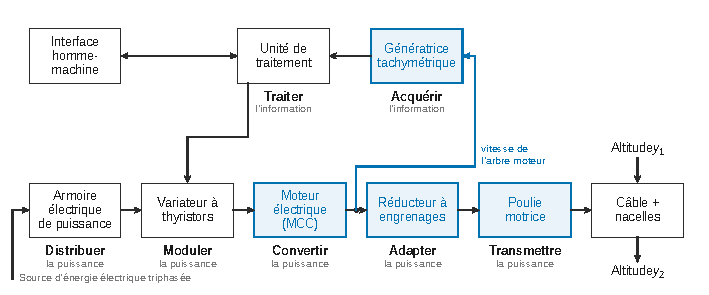
\includegraphics{figures/q03-chaines-fonctionnelles.pdf}
\caption*{Figure 1 --- DR1 complété : en bleu, les quatre constituants placés et
la mesure de vitesse prise sur l'arbre moteur}
\end{figure}

\hypertarget{q4}{%
\subsubsection{Q4}\label{q4}}

Non-glissement sur la poulie motrice et réducteur : \(v=\dfrac{D_h}{2}\,\omega_h\) et \(\omega_h=k_{\text{\text{réd}}}\,\omega_m\), d'où

\equationajustee{\begin{aligned}{}&\boxed{k_{tp}=k_{\text{\text{réd}}}\,\frac{D_h}{2}}\\
k_{tp}&=\frac{1}{60{,}07}\times\frac{4{,}6}{2}=\boxed{3{,}829\times10^{-2}\ \text{m}\cdot\text{rad}^{-1}}
\end{aligned}}

Les deux méthodes donnent \(3{,}8288\times10^{-2}\) (mesure, Q2) et \(3{,}8289\times10^{-2}\) (documentation), soit un écart relatif de \(3\times10^{-5}\) : \textbf{la valeur de Q2 est validée.}

\hypertarget{ii.2-configuration-de-secours}{%
\subsubsection{II.2 --- Configuration de secours}\label{ii.2-configuration-de-secours}}

\hypertarget{q5}{%
\subsubsection{Q5}\label{q5}}

Chaîne de secours : moteur diesel, réducteur \(k_r\), coupleur de rapport 1, réducteur principal \(k_{\text{\text{réd}}}\), poulie motrice. Donc \(v_s=k_r\,k_{tp}\,\omega_s\) :

\equationajustee{\begin{aligned}
\omega_s&=\frac{v_s}{k_r\,k_{tp}}=\frac{1{,}25\times7{,}04}{3{,}829\times10^{-2}}\\
&=229{,}8\ \text{rad}\cdot\text{s}^{-1}\\
N_s&=\frac{30}{\pi}\,\omega_s=\boxed{2195\ \text{tr}\cdot\text{min}^{-1}}
\end{aligned}}

\(N_s<N_{s\max}=3000\) tr/min : \textbf{la configuration de secours est compatible} avec le moteur thermique (marge de 27 \%).

\hypertarget{partie-b-uxe9tude-de-lexigence-id-1.1-guxe9rer-la-suxe9curituxe9-et-le-confort-des-usagers}{%
\section{Partie B --- Étude de l'exigence Id = 1.1 « gérer la sécurité et le confort des usagers »}\label{partie-b-uxe9tude-de-lexigence-id-1.1-guxe9rer-la-suxe9curituxe9-et-le-confort-des-usagers}}

\hypertarget{moteur-et-poulies}{%
\subsection{Moteur et poulies}\label{moteur-et-poulies}}

\hypertarget{q6}{%
\subsubsection{Q6}\label{q6}}

Rotor en rotation autour d'un axe fixe du référentiel galiléen, de moment d'inertie \(J_m\) autour de cet axe :

\equationajustee{\boxed{E_c(\text{mot}/0)=\tfrac12\,J_m\,\omega_m^2}.}

\hypertarget{q7}{%
\subsubsection{Q7}\label{q7}}

\equationajustee{\begin{aligned}{}&\boxed{E_c(\text{bas}/0)=\tfrac12\,J_b\,\omega_b^2}\\
&\boxed{E_c(\text{haut}/0)=\tfrac12\,J_h\,\omega_h^2}
\end{aligned}}

Avec \(\omega_h=k_{\text{\text{réd}}}\,\omega_m\) et \(D_b\,\omega_b=D_h\,\omega_h\), on obtient \(\omega_b=\dfrac{D_h}{D_b}k_{\text{\text{réd}}}\,\omega_m\).

L'égalité \(E_c(\text{bas}/0)+E_c(\text{haut}/0)=\tfrac12 J_{\text{\text{éq}-poulies}}\,\omega_m^2\) donne

\equationajustee{\begin{aligned}{}&\boxed{J_{\text{\text{éq}-poulies}}=k_{\text{\text{réd}}}^2\left[J_h+\left(\frac{D_h}{D_b}\right)^2J_b\right]}\\
J_{\text{\text{éq}-poulies}}&=2{,}771\times10^{-4}\times(25\,700+1{,}259\times16\,200)\\
&=12{,}8\ \text{kg}\cdot\text{m}^2
\end{aligned}}

\hypertarget{cuxe2ble-et-nacelles}{%
\subsection{Câble et nacelles}\label{cuxe2ble-et-nacelles}}

\hypertarget{q8}{%
\subsubsection{Q8}\label{q8}}

Chaque brin, de masse \(\lambda L_p\), est en translation à la vitesse \(v\) :

\equationajustee{\boxed{E_c(\text{mont}/0)=E_c(\text{desc}/0)=\tfrac12\,\lambda L_p\,v^2}.}

L'énergie cinétique étant quadratique en vitesse, les deux contributions s'ajoutent. Avec \(v=k_{tp}\,\omega_m\) :

\equationajustee{\begin{aligned}
\lambda L_p\,k_{tp}^2\,\omega_m^2&=\tfrac12\,J_{\text{\text{éq}-\text{câble}}}\,\omega_m^2\\
\Longrightarrow\quad&\boxed{J_{\text{\text{éq}-\text{câble}}}=2\,\lambda\,L_p\,k_{tp}^2}\\
J_{\text{\text{éq}-\text{câble}}}&=2\times7{,}81\times1217\times(3{,}829\times10^{-2})^2\\
&=27{,}9\ \text{kg}\cdot\text{m}^2
\end{aligned}}

\hypertarget{q9}{%
\subsubsection{Q9}\label{q9}}

Les \(N-6=66\) nacelles entraînées se répartissent en \(N/2-3=33\) montantes chargées et \(33\) descendantes vides, toutes en translation à la vitesse \(v\) :

\equationajustee{\begin{aligned}{}&\boxed{E_c(\text{mont}/0)=\tfrac12\left(\tfrac N2-3\right)(M_n+M_c)\,v^2}\\
&\boxed{E_c(\text{desc}/0)=\tfrac12\left(\tfrac N2-3\right)M_n\,v^2}
\end{aligned}}

En sommant, avec \(v=k_{tp}\,\omega_m\) :

\equationajustee{\begin{aligned}{}&\boxed{J_{\text{\text{éq}-nacelles}}=\left(\frac N2-3\right)(2M_n+M_c)\,k_{tp}^2}\\
J_{\text{\text{éq}-nacelles}}&=33\times870\times1{,}466\times10^{-3}\\
&=42{,}1\ \text{kg}\cdot\text{m}^2
\end{aligned}}

\hypertarget{ensemble-en-mouvement}{%
\subsection{Ensemble en mouvement}\label{ensemble-en-mouvement}}

\hypertarget{q10}{%
\subsubsection{Q10}\label{q10}}

Le moteur, les poulies, le câble et les nacelles forment l'ensemble mobile, dont l'énergie cinétique est la somme des énergies des parties (réducteur négligé) :

\equationajustee{J_{\text{\text{éq}}}=J_m+J_{\text{\text{éq}-poulies}}+J_{\text{\text{éq}-\text{câble}}}+J_{\text{\text{éq}-nacelles}}.}

Avec \(k_{tp}^2=k_{\text{\text{réd}}}^2D_h^2/4\) :

\equationajustee{J_{\text{\text{éq}}}=J_m+k_{\text{\text{réd}}}^2\left[J_h+\left(\frac{D_h}{D_b}\right)^2J_b+\frac{D_h^2}{2}\lambda L_p+(N-6)\frac{D_h^2}{4}M_n+(N-6)\frac{D_h^2}{8}M_c\right].}

La masse notée \(M_p\) dans la forme imposée est la masse de la charge \(M_c\) (seule grandeur restante). Par identification :

\equationajustee{\boxed{\begin{aligned}
\beta_1&=k_{\text{\text{réd}}}^2\\
\beta_2&=\left(\frac{D_h}{D_b}\right)^2\\
\mu_1&=\frac{D_h^2}{2}\\
\mu_2&=\frac{(N-6)\,D_h^2}{4}\\
\mu_3&=\frac{(N-6)\,D_h^2}{8}
\end{aligned}}}

Application numérique :

\begin{longtable}[]{@{}
  >{\raggedright\arraybackslash}p{(\columnwidth - 10\tabcolsep) * \real{0.1667}}
  >{\raggedright\arraybackslash}p{(\columnwidth - 10\tabcolsep) * \real{0.1667}}
  >{\raggedright\arraybackslash}p{(\columnwidth - 10\tabcolsep) * \real{0.1667}}
  >{\raggedright\arraybackslash}p{(\columnwidth - 10\tabcolsep) * \real{0.1667}}
  >{\raggedright\arraybackslash}p{(\columnwidth - 10\tabcolsep) * \real{0.1667}}
  >{\raggedright\arraybackslash}p{(\columnwidth - 10\tabcolsep) * \real{0.1667}}@{}}
\toprule\noalign{}
\begin{minipage}[b]{\linewidth}\raggedright
Coefficient
\end{minipage} & \begin{minipage}[b]{\linewidth}\raggedright
\(\beta_1\)
\end{minipage} & \begin{minipage}[b]{\linewidth}\raggedright
\(\beta_2\)
\end{minipage} & \begin{minipage}[b]{\linewidth}\raggedright
\(\mu_1\)
\end{minipage} & \begin{minipage}[b]{\linewidth}\raggedright
\(\mu_2\)
\end{minipage} & \begin{minipage}[b]{\linewidth}\raggedright
\(\mu_3\)
\end{minipage} \\
\midrule\noalign{}
\endhead
\bottomrule\noalign{}
\endlastfoot
Valeur & \(2{,}771\times10^{-4}\) & \(1{,}259\) & \(10{,}58\) m² & \(349{,}1\) m² & \(174{,}6\) m² \\
\end{longtable}

Le crochet vaut, en kg·m² :

\equationajustee{\begin{aligned}{}&25\,700+20\,392+100\,561+38\,405+113\,471\\
&=298\,529
\end{aligned}}

donc

\equationajustee{\begin{aligned}
J_{\text{\text{éq}}}&=23+2{,}771\times10^{-4}\times298\,529\\
&=23+82{,}7\\
&=\boxed{1{,}06\times10^2\ \text{kg}\cdot\text{m}^2}
\end{aligned}}

Répartition : rotor 23 ; poulies 12,8 ; câble 27,9 ; nacelles 10,6 ; charge 31,4 kg·m².

\hypertarget{puissance-des-actions-muxe9caniques-de-pesanteur}{%
\subsection{Puissance des actions mécaniques de pesanteur}\label{puissance-des-actions-muxe9caniques-de-pesanteur}}

\hypertarget{q11}{%
\subsubsection{Q11}\label{q11}}

Le câble est une boucle fermée de masse linéique uniforme. Au cours du défilement, la répartition de matière dans l'espace ne change pas : l'altitude de son centre de gravité est constante, donc son énergie potentielle aussi, et \(\mathscr P(\text{pes}\to\text{\text{câble}}/0)=-\dfrac{\mathrm dE_p}{\mathrm dt}=0\). Formulé brin par brin : les deux brins ont la même masse \(\lambda L_p\) et des vitesses opposées, donc des puissances de pesanteur opposées. \textbf{La puissance de la pesanteur sur le câble est nulle.}

\hypertarget{q12}{%
\subsubsection{Q12}\label{q12}}

Avec \(\vec g=-g\,\vec y_0\), une nacelle montante (masse \(M_n+M_c\)) a une vitesse verticale \(+v\sin\alpha\), une descendante (masse \(M_n\)) une vitesse verticale \(-v\sin\alpha\) :

\begin{figure}[H]
\centering
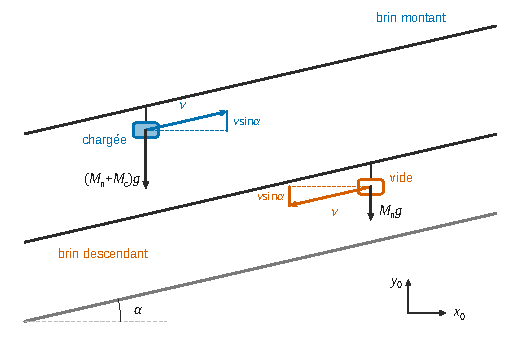
\includegraphics{figures/q12-pesanteur-nacelles.pdf}
\caption*{Figure 2 --- Pesanteur sur les nacelles : montante chargée et
descendante vide, de vitesses verticales opposées v sin α}
\end{figure}

\equationajustee{\begin{aligned}
\mathscr P(\text{pes}\to\text{nacelles}/0)&=\left(\tfrac N2-3\right)g\,v\sin\alpha\,\big[-(M_n+M_c)+M_n\big]\\
&=-\left(\tfrac N2-3\right)M_c\,g\,v\sin\alpha
\end{aligned}}

Avec \(v=k_{tp}\,\omega_m\) :

\equationajustee{\begin{aligned}{}&\boxed{\mathcal C=-\left(\frac N2-3\right)M_c\,g\,k_{tp}\,\sin\alpha}\\
\mathcal C&=-33\times650\times9{,}81\times3{,}829\times10^{-2}\times\sin12{,}9^\circ\\
&=\boxed{-1{,}80\times10^3\ \text{N}\cdot\text{m}}
\end{aligned}}

\hypertarget{uxe9valuation-de-la-puissance-moteur}{%
\subsection{Évaluation de la puissance moteur}\label{uxe9valuation-de-la-puissance-moteur}}

\hypertarget{q13}{%
\subsubsection{Q13}\label{q13}}

Théorème de l'énergie cinétique appliqué à \((\Sigma)\) dans le référentiel galiléen lié au sol :

\equationajustee{\frac{\mathrm dE_c(\Sigma/0)}{\mathrm dt}=\mathscr P(\bar\Sigma\to\Sigma/0)+\mathscr P_{\text{int}}(\Sigma)}

avec

\equationajustee{E_c(\Sigma/0)=\tfrac12\,J_{\text{\text{éq}}}\,\omega_m^2.}

Puissances extérieures : pesanteur nulle sur le câble (Q11) et sur les solides en rotation autour d'axes fixes (centres de gravité fixes), égale à \(\mathcal C\,\omega_m\) sur les nacelles (Q12) ; liaisons avec le bâti parfaites.

Puissances intérieures : liaisons parfaites, pas de glissement, pertes négligées ; il ne reste que la puissance motrice \(\mathscr P_{m\,\text{utile}}\). D'où

\equationajustee{J_{\text{\text{éq}}}\,\omega_m\,\dot\omega_m=\mathcal C\,\omega_m+\mathscr P_{m\,\text{utile}}.}

À vitesse constante :

\equationajustee{\boxed{\mathscr P_{m\,\text{utile}}=-\mathcal C\,\omega_m}\quad(>0\ \text{car}\ \mathcal C<0).}

\hypertarget{q14}{%
\subsubsection{Q14}\label{q14}}

Avec la valeur d'exploitation \(\mathcal C\simeq-900\) N·m et \(\omega_m=132{,}7\) rad/s :

\equationajustee{\begin{aligned}
\mathscr P_{m\,\text{utile}}&=900\times132{,}68=1{,}19\times10^5\ \text{W}\\
s&=\frac{\mathscr P_{m\,\text{nom}}}{\mathscr P_{m\,\text{utile}}}=\frac{415}{119{,}4}\\
&=\boxed{3{,}5}
\end{aligned}}

\(s>3\) : \textbf{l'exigence id = « 1.1 » est vérifiée.} Avec la charge limite (\(\mathcal C=-1{,}80\) kN·m, jamais atteinte), on aurait \(239\) kW et \(s=1{,}7\).

\hypertarget{partie-c-uxe9tude-de-lexigence-id-1.2-entrauxeener-le-cuxe2ble-et-les-nacelles-entre-les-gares}{%
\section{Partie C --- Étude de l'exigence Id = « 1.2 » « entraîner le câble et les nacelles entre les gares »}\label{partie-c-uxe9tude-de-lexigence-id-1.2-entrauxeener-le-cuxe2ble-et-les-nacelles-entre-les-gares}}

\hypertarget{i-estimation-des-grandeurs-de-la-machine-uxe0-courant-continu-en-charge}{%
\subsection{I --- Estimation des grandeurs de la machine à courant continu en charge}\label{i-estimation-des-grandeurs-de-la-machine-uxe0-courant-continu-en-charge}}

\hypertarget{i.1-mise-en-place-du-schuxe9ma-bloc}{%
\subsubsection{I.1 --- Mise en place du schéma-bloc}\label{i.1-mise-en-place-du-schuxe9ma-bloc}}

\hypertarget{q15}{%
\subsubsection{Q15}\label{q15}}

Équations simplifiées en Laplace (conditions initiales nulles) :

\equationajustee{\begin{aligned}
U_m&=R\,I+E\\
J_{\text{\text{éq}}}\,p\,\Omega_m&=C_m+C_r\\
E&=k\,\Omega_m\\
C_m&=k\,I
\end{aligned}}

Schéma DR2 complété (figure 3) :

\begin{itemize}
\tightlist
\item
  comparateur \(U_m(p)-E(p)\), puis blocs \(\dfrac1R\) et \(k\) ;
\item
  sommateur \(C_m(p)+C_r(p)\), puis bloc \(\dfrac1{J_{\text{\text{éq}}}\,p}\) ;
\item
  retour \(k\) qui forme \(E(p)=k\,\Omega_m(p)\).
\end{itemize}

\begin{figure}[H]
\centering
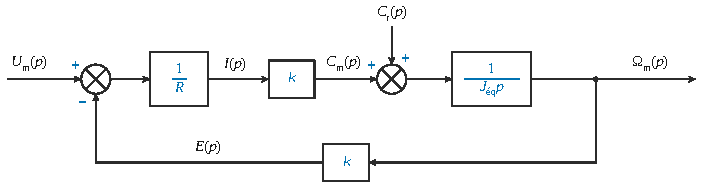
\includegraphics{figures/q15-schema-bloc-mcc.pdf}
\caption*{Figure 3 --- DR2 complété : schéma-bloc de la MCC, en bleu les blocs et
les signes ajoutés}
\end{figure}

Résolution : \(\left(J_{\text{\text{éq}}}\,p+\dfrac{k^2}{R}\right)\Omega_m=\dfrac kR\,U_m+C_r\), d'où

\equationajustee{\boxed{\begin{aligned}
H_m(p)&=\frac{K_m}{1+T_m\,p}\\
H_r(p)&=\frac{K_r}{1+T_m\,p}\\
K_m&=\frac1k\\
K_r&=\frac R{k^2}\\
T_m&=\frac{R\,J_{\text{\text{éq}}}}{k^2}
\end{aligned}}}

Unités : \(K_m\) en rad·s⁻¹·V⁻¹, \(K_r\) en rad·s⁻¹·N⁻¹·m⁻¹, \(T_m\) en s.

Avec \(R=15\) mΩ, \(k=3\) N·m/A et \(J_{\text{\text{éq}}}\approx106\) kg·m² :

\begin{itemize}
\tightlist
\item
  \(K_m=0{,}33\) rad·s⁻¹·V⁻¹ ;
\item
  \(K_r=1{,}7\times10^{-3}\) rad·s⁻¹·N⁻¹·m⁻¹ ;
\item
  \(T_m\approx0{,}18\) s.
\end{itemize}

\hypertarget{i.2-estimation-des-grandeurs-du-moduxe8le-par-des-mesures-sur-site}{%
\subsubsection{I.2 --- Estimation des grandeurs du modèle par des mesures sur site}\label{i.2-estimation-des-grandeurs-du-moduxe8le-par-des-mesures-sur-site}}

\hypertarget{q16}{%
\subsubsection{Q16}\label{q16}}

En régime permanent, \(u_m=R\,i+k\,\omega_m\) avec \(\omega_1=840\pi/30=87{,}96\) rad/s et \(\omega_2=1267\pi/30=132{,}68\) rad/s :

\equationajustee{\boxed{\begin{aligned}
A&=\begin{pmatrix}284{,}9&87{,}96\\429{,}7&132{,}68\end{pmatrix}\\
X&=\begin{pmatrix}R\\k\end{pmatrix}\\
B&=\begin{pmatrix}265{,}2\\400{,}0\end{pmatrix}
\end{aligned}}}

Lignes à compléter sur DR3 :

\begin{lstlisting}[language=Python]
import numpy as np
A = np.array([[284.9, 840*np.pi/30], [429.7, 1267*np.pi/30]])
B = np.array([265.2, 400.0])
X = np.linalg.solve(A, B)
\end{lstlisting}

Résultat : \(X\approx(0{,}41\ ;\ 1{,}67)\), soit \(R\approx0{,}4\ \Omega\) et \(k\approx1{,}7\) N·m/A.

Les deux lignes sont presque proportionnelles (\(\det A\approx2{,}1\), minuscule devant les produits de coefficients, de l'ordre de \(4\times10^4\)). Le résultat est donc extrêmement sensible aux arrondis :

\begin{itemize}
\tightlist
\item
  avec \(87{,}96\) et \(132{,}68\) rad/s, on trouve \(R=0{,}66\) et \(k=0{,}86\) ;
\item
  avec \(88{,}0\) et \(132{,}7\) rad/s, on trouve \(k<0\).
\end{itemize}

Ce calcul ne fournit donc qu'un ordre de grandeur, d'où les valeurs moyennes \(R=15\) mΩ et \(k=3\) N·m/A retenues ensuite.

\hypertarget{q17}{%
\subsubsection{Q17}\label{q17}}

Sur \([0\,;t_f]\), \(N_m\) décroît linéairement de \(N_0\) à \(0\) :

\equationajustee{\boxed{\frac{\mathrm d\omega_m}{\mathrm dt}=-\frac{\pi\,N_0}{30\,t_f}}\quad\text{(constante)}.}

Alimentation coupée : \(i=0\) donc \(c_m=0\), et l'équation complète serait

\equationajustee{J_{\text{\text{éq}}}\,\dot\omega_m=c_r-f_{\text{\text{éq}}}\,\omega_m.}

Avec un frottement visqueux non négligeable, la décélération dépendrait de \(\omega_m\) et la vitesse décroîtrait selon une exponentielle (courbe convexe, à pente de moins en moins forte). La décroissance observée est linéaire : \textbf{le terme \(f_{\text{\text{éq}}}\,\omega_m\) est négligeable, ce qui confirme l'hypothèse faite sur \((E_2)\).}

\hypertarget{q18}{%
\subsubsection{Q18}\label{q18}}

Avec \(c_m=0\), \(f_{\text{\text{éq}}}\) négligé et \(c_r=c_{r0}\) constant, l'équation \((E_2)\) s'intègre :

\equationajustee{\begin{aligned}
J_{\text{\text{éq}}}\,\dot\omega_m&=c_{r0}\\
\omega_m(t)&=\omega_0+\frac{c_{r0}}{J_{\text{\text{éq}}}}\,t
\end{aligned}}

En tours par minute (\(N=30\,\omega/\pi\)) :

\equationajustee{\boxed{N_m(t)=\frac{30\,c_{r0}}{\pi\,J_{\text{\text{éq}}}}\,t+N_0}\qquad(c_{r0}<0).}

\hypertarget{q19}{%
\subsubsection{Q19}\label{q19}}

Avant \(t=0\), en régime stabilisé : \(0=k\,I(0^-)+c_{r0}\), soit \(\boxed{c_{r0}=-k\,I(0^-)}\) :

\equationajustee{\begin{aligned}
c_{r0\text{-v}}&=-3\times360=\boxed{-1{,}08\times10^3\ \text{N}\cdot\text{m}}\\
c_{r0\text{-c}}&=-3\times520=\boxed{-1{,}56\times10^3\ \text{N}\cdot\text{m}}
\end{aligned}}

\(N_m(t_f)=0\) donne

\equationajustee{\begin{aligned}
J_{\text{\text{éq}}}&=-\frac{30\,c_{r0}\,t_f}{\pi\,N_0}\\
&=\boxed{\frac{k\,I(0^-)\,t_f}{\omega_0}}
\end{aligned}}

\equationajustee{\begin{aligned}
J_{\text{\text{éq}-v}}&=\frac{1080\times10{,}3}{132{,}68}=\boxed{84\ \text{kg}\cdot\text{m}^2}\\
J_{\text{\text{éq}-c}}&=\frac{1560\times8{,}9}{132{,}68}=\boxed{105\ \text{kg}\cdot\text{m}^2}
\end{aligned}}

La valeur en charge recoupe à 1 \% le calcul théorique de Q10 (106 kg·m², nacelles pleines).

\hypertarget{ii-obtention-de-la-vitesse-angulaire-depuis-la-mesure-de-position}{%
\subsection{II --- Obtention de la vitesse angulaire depuis la mesure de position}\label{ii-obtention-de-la-vitesse-angulaire-depuis-la-mesure-de-position}}

\hypertarget{q20}{%
\subsubsection{Q20}\label{q20}}

Une dynamo tachymétrique est une petite génératrice à courant continu à flux inducteur constant (aimants permanents), dont l'induit est entraîné par l'arbre moteur. Les conducteurs de l'induit coupent le flux fixe : il y apparaît une f.é.m. induite proportionnelle à la vitesse, redressée par le collecteur. Débitant un courant quasi nul, elle délivre une tension \(u=k_{\text{dt}}\,N_m\), image de la vitesse et de signe lié au sens de rotation.

\hypertarget{q21}{%
\subsubsection{Q21}\label{q21}}

Lecture du signal brut : valeur moyenne \(\approx76\) V (cohérent avec \(0{,}06\times1267=76\) V), extrêmes \(\approx69\) V et \(\approx82\) V, soit un écart d'environ \(\pm6{,}5\) V autour de la moyenne. Avec \(k_{\text{dt}}=0{,}06\) V·min·tr⁻¹ :

\equationajustee{\begin{aligned}
\Delta N_m&=\frac{\pm6{,}5}{0{,}06}\approx\boxed{\pm1{,}1\times10^2\ \text{tr}\cdot\text{min}^{-1}}\\
\left|\frac{\Delta v}{v}\right|&=\frac{\Delta N_m}{N_m}=\frac{108}{1267}\\
&\approx\boxed{8{,}5\ \%}
\end{aligned}}

(17 \% en crête à crête). La chaîne cinématique ayant un gain constant, la fluctuation relative de \(v\) est celle de \(N_m\). \textbf{Elle dépasse l'exigence \(|\Delta v/v|<5\ \%\)} : le signal brut est inexploitable. Il s'agit surtout de bruit de mesure (l'inertie de l'installation interdit de telles variations réelles en quelques millisecondes) ; le signal filtré reste dans une bande d'environ \(\pm0{,}6\) V, soit moins de 1 \%.

\hypertarget{q22}{%
\subsubsection{Q22}\label{q22}}

\(U^*(p)\,(1+2\tau p+\tau^2p^2)=U(p)\), d'où, à conditions initiales nulles,

\equationajustee{\boxed{\tau^2\,\ddot u^*(t)+2\tau\,\dot u^*(t)+u^*(t)=u(t)}.}

\hypertarget{q23}{%
\subsubsection{Q23}\label{q23}}

Schéma « à gauche » appliqué deux fois : \(\dot u^*_i=\dfrac{u^*_i-u^*_{i-1}}{T_e}\) et \(\ddot u^*_i=\dfrac{u^*_i-2u^*_{i-1}+u^*_{i-2}}{T_e^2}\). En reportant, avec \(x=\tau/T_e\) :

\equationajustee{\begin{aligned}{}&x^2\,(u^*_i-2u^*_{i-1}+u^*_{i-2})+2x\,(u^*_i-u^*_{i-1})+u^*_i=u_i\\
\Longrightarrow\quad&(1+x)^2\,u^*_i=u_i+2x(1+x)\,u^*_{i-1}-x^2\,u^*_{i-2}
\end{aligned}}

\equationajustee{\boxed{\begin{aligned}
u^*_i&=a_0\,u_i+a_1\,u^*_{i-1}+a_2\,u^*_{i-2}\\
a_0&=\frac1{(1+x)^2}\\
a_1&=\frac{2x}{1+x}\\
a_2&=-\frac{x^2}{(1+x)^2}
\end{aligned}}}

Contrôle : \(a_0+a_1+a_2=1\) (gain statique unitaire).

\hypertarget{q24}{%
\subsubsection{Q24}\label{q24}}

Avantage principal : \textbf{la souplesse de réglage}. Les coefficients \(a_0\), \(a_1\), \(a_2\) sont des nombres programmés ; on modifie \(\tau\) par logiciel sans toucher au matériel, et le filtre ne dérive pas avec le vieillissement ou la température des composants.

\hypertarget{iii-pilotage-du-moteur-en-phase-de-duxe9marrage-en-charge-maximale}{%
\subsection{III --- Pilotage du moteur en phase de démarrage en charge maximale}\label{iii-pilotage-du-moteur-en-phase-de-duxe9marrage-en-charge-maximale}}

\hypertarget{iii.1-duxe9termination-de-la-capacituxe9-en-courant-du-variateur-implantuxe9}{%
\subsubsection{III.1 --- Détermination de la capacité en courant du variateur implanté}\label{iii.1-duxe9termination-de-la-capacituxe9-en-courant-du-variateur-implantuxe9}}

\hypertarget{q25}{%
\subsubsection{Q25}\label{q25}}

\begin{itemize}
\tightlist
\item
  Pour \(t\in[0\,;t_{acc}]\) : \(v(t)=\gamma_{\max}\,t\) (rampe).
\item
  Pour \(t\geqslant t_{acc}\) : \(v=v_n\) (palier).
\end{itemize}

Allure : segment de droite de l'origine au point \((t_{acc}\,;5{,}08\ \text{m/s})\), puis horizontale.

\equationajustee{\begin{aligned}
t_{acc}&=\frac{v_n}{\gamma_{\max}}=\frac{5{,}08}{0{,}5}\\
&=\boxed{10{,}16\ \text{s}}
\end{aligned}}

L'exigence « accélération douce : \(t_{acc}>10\) s » (portée par l'exigence 1.1 de la figure 2) est \textbf{vérifiée, de justesse} (1,6 \% de marge).

\hypertarget{q26}{%
\subsubsection{Q26}\label{q26}}

\equationajustee{i=\frac{M_{\text{\text{éq}}}\,k_{tp}\,\gamma+c_r}{k}}

avec \(M_{\text{\text{éq}}}=65\) t, \(k_{tp}=0{,}040\) m/rad, \(c_r=1800\) N·m et \(k=3\) N·m/A.

\begin{itemize}
\tightlist
\item
  Phase 1 (\(0\leqslant t\leqslant t_{acc}\), \(\gamma=0{,}5\) m/s²) :
\end{itemize}

\equationajustee{\begin{aligned}
i_1&=\frac{65\,000\times0{,}040\times0{,}5+1800}{3}\\
&=\frac{1300+1800}{3}\\
&=\boxed{1033\ \text{A}}
\end{aligned}}

\begin{itemize}
\tightlist
\item
  Phase 2 (\(t\geqslant t_{acc}\), \(\gamma=0\)) : \(i_2=\dfrac{1800}3=\boxed{600\ \text{A}}\).
\end{itemize}

Allure (figure 4) : palier à 1033 A jusqu'à \(t_{acc}=10{,}16\) s, puis palier à 600 A.

\(i_{\max}=1033\ \text{A}<i_{\text{nom}}=1064\) A : \textbf{l'intensité maximale n'est jamais atteinte} (marge de 3 \%).

\begin{figure}[H]
\centering
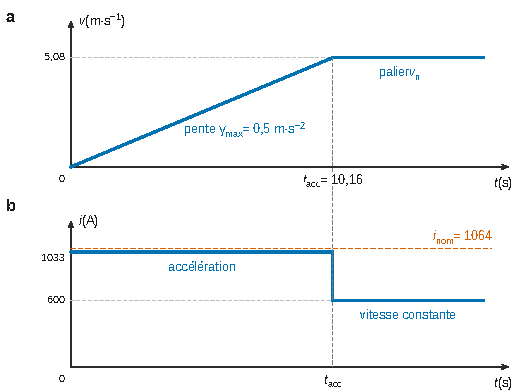
\includegraphics{figures/q25-q26-demarrage.pdf}
\caption*{Figure 4 --- Démarrage en charge maximale : vitesse v(t) des nacelles et
intensité i(t), toujours sous le courant nominal de 1064 A}
\end{figure}

\hypertarget{iii.2-du-variateur-actuellement-implantuxe9-uxe0-une-nouvelle-technologie-de-motorisation}{%
\subsubsection{III.2 --- Du variateur actuellement implanté à une nouvelle technologie de motorisation}\label{iii.2-du-variateur-actuellement-implantuxe9-uxe0-une-nouvelle-technologie-de-motorisation}}

\hypertarget{q27}{%
\subsubsection{Q27}\label{q27}}

\(U_{\max}\) est la tension composée maximale : \(U_{\max}=\sqrt2\times391=553\) V. Avec \(\langle U_m\rangle=u_{m\,\text{nom}}=400\) V :

\equationajustee{\begin{aligned}
\cos\psi&=\frac{400\,\pi}{3\times553}=0{,}757\\
\Longrightarrow\quad&\boxed{\psi=0{,}71\ \text{rad}\ (41^\circ)}
\end{aligned}}

\hypertarget{q28}{%
\subsubsection{Q28}\label{q28}}

En régime permanent, \(\langle U_m\rangle=R\,I+k\,\Omega_m\), donc

\equationajustee{\boxed{N_{m\text{-rp}}=\frac{30}{\pi\,k}\left(\frac3\pi\,U_{\max}\cos\psi-R\,I\right)}.}

\hypertarget{q29}{%
\subsubsection{Q29}\label{q29}}

Réseau à 50 Hz, période \(T=20\) ms (abscisses en ms).

\begin{itemize}
\tightlist
\item
  \textbf{Courbe A} : arches de sinusoïde toujours positives, s'annulant toutes les 10 ms (\(T/2\)), crête \(\approx320\) V (\(=\sqrt2\times226\) V), sans retard à la conduction. C'est un \textbf{redresseur monophasé double alternance non commandé} (pont PD2 à diodes) : \textbf{c'est la courbe de l'inducteur.}
\item
  \textbf{Courbe C} : tension comprise entre \(553\cos30^\circ\approx479\) V et \(\sqrt2\times391=553\) V. L'ondulation a pour période \(T/6=3{,}33\) ms et la valeur moyenne vaut \(\tfrac3\pi\times553=528\) V. C'est un \textbf{redresseur triphasé PD3} (à diodes, ou à thyristors avec \(\psi=0\)), structure du variateur d'induit.
\item
  \textbf{Courbe B} : créneaux à fronts verticaux alternant entre \(\approx+335\) V et \(\approx-335\) V, de période 10 ms, à valeur moyenne positive : \textbf{convertisseur à découpage}, hacheur réversible en pont (quatre quadrants) ou onduleur.
\end{itemize}

\hypertarget{q30}{%
\subsubsection{Q30}\label{q30}}

Pour la MCC :

\equationajustee{\begin{aligned}
\Omega_m&=\frac{\langle U_m\rangle-R\,I}{k}\\
\langle U_m\rangle&=\frac3\pi U_{\max}\cos\psi
\end{aligned}}

À \(U_{\max}\) imposé par le réseau, \textbf{le paramètre de réglage est l'angle de retard à l'amorçage \(\psi\)} (donc la tension moyenne d'induit).

Pour la MAS, la vitesse est voisine de la vitesse de synchronisme \(\Omega_s=2\pi f/p\) (\(p\) paires de pôles). Elle vaut \(\Omega=(1-g)\,\Omega_s\), avec un glissement \(g\) faible imposé par la charge. \textbf{Ce n'est donc pas le même paramètre : il faut agir sur la fréquence \(f\) des tensions statoriques}, en maintenant \(U/f\) constant pour conserver le flux. Le redresseur commandé doit être remplacé par un variateur de fréquence (redresseur, bus continu, onduleur triphasé MLI).

\hypertarget{q31}{%
\subsubsection{Q31}\label{q31}}

Le couple maximal d'une MAS est proportionnel au carré du flux, donc à \((U/f)^2\), et ne dépend pas de la fréquence si \(U/f\) est constant. Stratégie : \textbf{commande à \(U/f\) constant}, en démarrant à basse fréquence (vitesse de synchronisme faible, glissement voisin de celui du couple maximal dès l'arrêt), puis en augmentant progressivement la fréquence et la tension en proportion ; on ajoute une légère surtension à basse fréquence pour compenser la chute ohmique statorique. Le moteur développe ainsi son couple maximal pendant tout le démarrage, avec un courant limité par le variateur, bien inférieur à celui d'un démarrage direct.

\hypertarget{partie-d-uxe9tude-de-la-sous-exigence-maintenir-la-vitesse-des-nacelles-la-plus-ruxe9guliuxe8re-possible-de-lexigence-1.2}{%
\section{Partie D --- Étude de la sous-exigence « maintenir la vitesse des nacelles la plus régulière possible » de l'exigence 1.2}\label{partie-d-uxe9tude-de-la-sous-exigence-maintenir-la-vitesse-des-nacelles-la-plus-ruxe9guliuxe8re-possible-de-lexigence-1.2}}

\hypertarget{q32}{%
\subsubsection{Q32}\label{q32}}

Filtre de gain unitaire :

\equationajustee{\begin{aligned}
\varepsilon&=k_{\text{ad}}\,V_c-k_{\text{dt}}\,\Omega_m\\
V&=k_{\text{\text{réd}}}\frac{D_h}2\,\Omega_m\\
&=k_{tp}\,\Omega_m
\end{aligned}}

La condition \(\varepsilon=0\) pour \(V=V_c\) impose

\equationajustee{\boxed{k_{\text{ad}}=\frac{k_{\text{dt}}}{k_{tp}}=\frac{2\,k_{\text{dt}}}{k_{\text{\text{réd}}}\,D_h}}.}

Avec \(k_{\text{dt}}=0{,}06\) V·min·tr⁻¹ \(=0{,}06\times30/\pi=0{,}573\) V·s·rad⁻¹ : \(k_{\text{ad}}=0{,}573/0{,}03829=15{,}0\) V·s·m⁻¹.

\hypertarget{q33}{%
\subsubsection{Q33}\label{q33}}

Boucle ouverte (de \(\varepsilon\) au retour), \(C(p)=1\), \(C_r=0\) :

\equationajustee{\boxed{H_{bo}(p)=H_{\text{var}}(p)\,H_m(p)\,k_{\text{dt}}=\frac{K_v\,k_{\text{dt}}/k}{\left(1+\frac{T_v}2\,p\right)\left(1+T_m\,p\right)}}.}

Aucun pôle à l'origine : \textbf{\(H_{bo}\) est de classe 0} (ordre 2).

\hypertarget{q34}{%
\subsubsection{Q34}\label{q34}}

Classes : \(C_1\) donne une boucle ouverte de classe 0. Les deux autres correcteurs,

\equationajustee{\begin{aligned}
C_2&=K_p\frac{1+T_ip}{T_ip}\\
C_3&=\frac{K_p}p\cdot\frac{1+(T_f+T_d)p}{1+T_fp}
\end{aligned}}

donnent une classe 1, l'intégrateur étant situé dans le correcteur, en amont du point d'entrée de \(C_r\).

\begin{itemize}
\tightlist
\item
  Consigne en échelon : \(\zeta_\infty=\lim_{p\to0}\dfrac{v_0}{1+H_{bo}(p)}\) est nulle pour une classe \(\geqslant1\). \(C_1\) échoue ; \(C_2\) et \(C_3\) conviennent.
\item
  Perturbation constante \(C_r=c_0/p\) : \(v_\infty=\lim_{p\to0}\dfrac{k_{tp}\,K_r\,c_0}{1+H_{bo}(p)}\) est nulle dès qu'un intégrateur est placé en amont de la perturbation. \(C_1\) échoue ; \(C_2\) et \(C_3\) conviennent.
\end{itemize}

\textbf{Les correcteurs \(C_2\) et \(C_3\) respectent les exigences du cahier des charges, pas \(C_1\).} Si l'on exigeait en plus un écart nul pour une rampe de vitesse (accélération constante), il faudrait une classe 2, ce qu'aucun des trois candidats n'apporte. L'écart de traînage, \(\zeta_\infty=a/K\), reste alors faible (\(\approx0{,}14\) m/s pour \(a=0{,}5\) m/s² avec le réglage de Q35) et ne dure que le temps de l'accélération.

\hypertarget{q35}{%
\subsubsection{Q35}\label{q35}}

Avec \(T_i=T_v/2\), le zéro de \(C_2\) compense le pôle du variateur :

\equationajustee{H_{bo}(p)=\frac{K_p\,K_v\,k_{\text{dt}}}{k\,T_i}\,\frac1{p\,(1+T_m\,p)}.}

Le Bode de DR5 le confirme : pente \(-20\) puis \(-40\) dB/déc, phase de \(-90^\circ\) vers \(-180^\circ\).

\begin{itemize}
\tightlist
\item
  \textbf{Marge de gain} : la phase n'atteint \(-180^\circ\) qu'à l'infini, donc \(M_G=+\infty\). La condition \(M_G\geqslant12\) dB est vérifiée pour tout \(K_p>0\).
\item
  \textbf{Marge de phase} : il faut \(\varphi(\omega_{c0})\geqslant-120^\circ\). Tracés à laisser sur DR5 :

  \begin{itemize}
  \tightlist
  \item
    droite horizontale à \(-120^\circ\) sur la phase, coupée en \(\omega_{60}\approx3\) rad/s ;
  \item
    verticale jusqu'au diagramme de gain, où l'on lit \(G_{\text{dB}}(\omega_{60})\approx-6{,}8\) dB pour \(K_p=1\) ;
  \item
    translation de la courbe de gain de \(+6{,}8\) dB pour amener la coupure en \(\omega_{60}\).
  \end{itemize}
\end{itemize}

\begin{figure}[H]
\centering
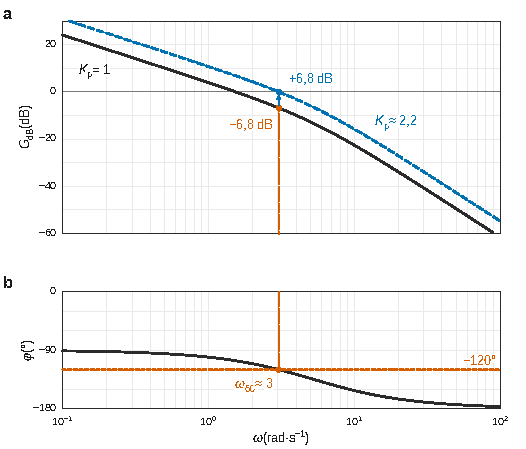
\includegraphics{figures/q35-bode-reglage-kp.pdf}
\caption*{Figure 5 --- Réglage de Kp sur le Bode : φ = −120° en ω60 ≈ 3 rad/s,
gain relevé de 6,8 dB}
\end{figure}

\equationajustee{20\log K_p=6{,}8\ \text{dB}\ \Longrightarrow\ \boxed{K_p\approx2{,}2}.}

La marge de phase diminue quand \(K_p\) augmente : les marges imposent \(K_p\leqslant2{,}2\) environ (2,2 à 2,4 selon la précision de lecture). La valeur limite \(K_p\approx2{,}2\) est la plus grande valeur admissible, donc le réglage le plus rapide et le plus précis qui respecte \(M_\varphi\geqslant60^\circ\).

\hypertarget{partie-e-synthuxe8se}{%
\section{Partie E --- Synthèse}\label{partie-e-synthuxe8se}}

\hypertarget{q36}{%
\subsubsection{Q36}\label{q36}}

La MCC alimente un induit tournant par un \textbf{collecteur et des balais} frottants, qui s'usent et imposent remplacements, nettoyage et rectification. La MAS à cage n'a aucun contact électrique glissant : \textbf{avantage principal, la suppression du système balais-collecteur, d'où une maintenance très réduite.}

\hypertarget{q37}{%
\subsubsection{Q37}\label{q37}}

\textbf{(a) Choix du moteur.} La puissance à fournir est fixée par la charge : \(\mathscr P_{m\,\text{utile}}=119{,}4\) kW (Q14). L'exigence \(s>3\) impose \(\mathscr P_{\text{nom}}>358\) kW. Pour la vitesse, la famille 4 pôles (1490 tr/min) est la plus proche du régime actuel (1267 tr/min) ; les 2 pôles (2980 tr/min) et les 6 pôles (960--995 tr/min) imposeraient une modification beaucoup plus forte de la réduction. Dans la famille 4 pôles, 315 kW (\(s=2{,}64\)) et 355 kW (\(s=2{,}97\)) sont insuffisants ; le premier moteur convenable est le

\equationajustee{\boxed{\text{GMM2E 355 L 4d : }400\ \text{kW},\ 1490\ \text{tr/min},\ 2563{,}8\ \text{N}\cdot\text{m},\ 710\ \text{A}}.}

Contrôle en couple : en régime établi d'exploitation, \(119\,400/156{,}0=765\) N·m, très en dessous du couple nominal. Au démarrage le plus contraignant (Q26), le couple \(k\,i_{\max}\approx3{,}1\) kN·m sur l'arbre actuel devient \(\approx3{,}1\times60{,}07/70{,}6\approx2{,}64\) kN·m avec le réducteur adapté du volet (d), soit 3 \% au-dessus du couple nominal pendant 10 s. La surcharge transitoire admissible d'une MAS pilotée en \(U/f\) le couvre. Un dimensionnement sans aucune surcharge conduirait au GMM 355 L 4e (450 kW, 2884 N·m).

\textbf{(b) Couplage.} Moteur 400 V/690 V : chaque enroulement supporte 400 V. Le réseau est en 226 V/391 V. En triangle, chaque enroulement reçoit la tension composée 391 V, soit environ sa tension nominale ; en étoile il ne recevrait que 226 V. \(\boxed{\text{Couplage triangle}}\).

\textbf{(c) Facteur de sécurité et conclusion.}

\equationajustee{s=\frac{400}{119{,}4}=\boxed{3{,}35>3}.}

L'exigence 1.1 est respectée, avec une marge proche de celle du moteur actuel (\(s=3{,}5\)). Sans contrainte d'implantation, \textbf{l'évolution vers la MAS est pertinente} : maintenance réduite (Q36), rendement de 95 \%, inertie rotorique plus faible (7,2 contre 23 kg·m²), puissance installée légèrement plus faible pour une sécurité de dimensionnement conservée, variation de vitesse assurée par un variateur de fréquence.

\textbf{(d) Modification de la chaîne de puissance.} Avec le réducteur actuel, 1490 tr/min donneraient \(v=0{,}03829\times156{,}0=5{,}97\) m/s, soit 18 \% de trop ; pour obtenir \(v_n\) il faudrait alimenter à \(\approx42{,}5\) Hz, hors du point nominal. Pour que le moteur fonctionne autour de sa vitesse nominale (glissement nominal, \(g=(1500-1490)/1500=0{,}67\ \%\)) quand le câble est à \(v_n\), il faut :

\begin{itemize}
\tightlist
\item
  \textbf{remplacer le réducteur principal} par un réducteur de rapport \(k'_{\text{\text{réd}}}=\dfrac{2\,v_n}{D_h\,\omega_{\text{nom}}}=\dfrac{5{,}08}{2{,}3\times156{,}0}=\boxed{\dfrac1{70{,}6}}\) (au lieu de \(1/60{,}07\)) ;
\item
  \textbf{remplacer le variateur à thyristors par un variateur de fréquence} (redresseur, bus continu, onduleur MLI), alimenté par le réseau triphasé, qui gère les démarrages, les arrêts et la vitesse réduite.
\end{itemize}

\end{document}
